\clearpage
\setcounter{page}{1}
\maketitlesupplementary

\section{3D Feature Uplifting as Maximum Likelihood Estimation}
Our weighted feature uplifting formula is strongly grounded in the forward rendering process from a probabilistic perspective: Given the task of estimating 3d features $\mathbf{f} \in \mathbb{R}^d$ from a set of observed 2D features $\mathbf{F}^{2D} \in \mathbb{R}^d$, the Maximum-a-Posteriori~(MAP) estimator of 3D features $\mathbf{f}$ is
\begin{equation}
    \arg\max_\mathbf{f} p(\mathbf{f}|\mathbf{F}^{2D}) = \arg\max_\mathbf{f} p(\mathbf{F}^{2D}|\mathbf{f})\frac{p(\mathbf{f})}{p(\mathbf{F}^{2D})},
    \label{eq:map}
\end{equation}
which forms the basis of our method.

\paragraph{Preliminaries}

Given the LGS setting, we make the following key assumptions about the feature uplifting problem.

\begin{enumerate}[label=(\roman*)]
    \item \textbf{Uniform Prior}: The language features in CLIP space have uniform distribution, which is motivated by the efficient use of the CLIP feature space, due to training of a large amount of diverse data
    \begin{equation}
        p(\mathbf{f}) \propto \text{constant}.
        \label{eq:uniform_clip}
    \end{equation}
    
    \item \textbf{Conditional Independence of pixels}: Pixel observations are conditionally independent given the surface representation and 3D features $\mathbf{f}$
    \begin{equation}
        p(\mathbf{F}^{2D}|\mathbf{f}) = \prod_{v=1}^V \prod_{p \in P_v} p(\mathbf{f}_{p,v}^{2D}|\mathbf{f}).
        \label{eq:cond_ind}
    \end{equation}
    where $\mathbf{f}_{p,v}^{2D}$ denotes the 2D feature at pixel $p$ in view $v$.
    
    \item \textbf{Gaussian feature noise}: Viewpoint dependency of CLIP features can be modeled by a Gaussian distribution of feature noise
    \begin{equation}
        \epsilon_{p,v} \sim \mathcal{N}(\mathbf{0}, \sigma^2\mathbf{I}).
    \end{equation}
    
    \item \textbf{Alpha Blending Weights}: Alpha blending weights applied to each Gaussian $i$ at pixel $p$ in view $v$ can be interpreted as measures of occlusion between separate Gaussians in a given camera view
    \begin{equation}
        w_{i,p,v} = \alpha_i \prod_{j=1}^{i-1}(1-\alpha_j).
        \label{eq:alpha_blending}
    \end{equation}    
\end{enumerate}

\paragraph{Occam's LGS as a MAP estimator}
Our approach formulates feature uplifting as a MAP estimation problem, as stated in Equation~\ref{eq:map}. With the use of CLIP as language features, a model trained of large amounts of data is chosen. Under this condition, we make the assumption of a uniformly distributed feature space in Equation~\ref{eq:uniform_clip}. Under this condition, the LGS estimator is equivalent to the Maximum Likelihood~(ML)
\begin{equation}
    \arg\max_\mathbf{f} p(\mathbf{F}^{2D}|\mathbf{f}).
\end{equation}

This estimator can be evaluated separately for each 2D feature $\mathbf{f}_{p,v}^{2D}$ at pixel $p$ in view $v$ under conditional independence from Equation~\ref{eq:cond_ind}, given the surface representation and features $\mathbf{f}$ from the pretrained 3D Guassians
\begin{equation}
     \arg\max_\mathbf{f} p(\mathbf{F}^{2D}|\mathbf{f}) =  \arg\max_\mathbf{f} \prod_{v=1}^V \prod_{p \in P_v} p(\mathbf{f}_{p,v}^{2D}|\mathbf{f})
\end{equation}
where $P_v$ is the set of pixels in view $v$ on which Gaussian influences.

A major challenge in all LGS approaches is the viewpoint-dependent noise of 2D language features due to varying object appearance. Our approach formulates the ML estimation of LGS from noisy 2D features as IID normal distributed $\epsilon_{p,v} \sim \mathcal{N}(\mathbf{0}, \sigma^2\mathbf{I})$, representing the inherent uncertainty in the 2D features.

Hence, the 2D feature at pixel $p$ in view $v$, obtained from rendering the 3D Guassian features, is
\begin{equation}
    \mathbf{f}_{p,v}^{2D} = \sum_{k=1}^R w_{k,p,v}\mathbf{f}_k + \epsilon_{p,v},
\end{equation}
where $R$ is the number of Gaussians along the ray, $\epsilon_{p,v}$ is the language feature noise, and $w_{k,p,v}$ is the alpha blending weight for Gaussian $k$ at pixel $p$ in view $v$ defined in Equation~\ref{eq:alpha_blending}

To approach the ML estimation problem $\arg\max_\mathbf{f} p(\mathbf{F}^{2D}|\mathbf{f})$, we transform the problem to the log-likelihood domain
\begin{equation}
    \begin{aligned}
        &\log p(\mathbf{F}^{2D}|\mathbf{f}) = \log \prod_{v=1}^V \prod_{p \in P_v} p(\mathbf{f}_{p,v}^{2D}|\mathbf{f}) =\\
        &-\frac{1}{2\sigma^2} \sum_{v,p} \left\| \mathbf{f}_{p,v}^{2D} - \sum_{k=1}^R w_{k,p,v}\mathbf{f}_k \right\|^2 + \text{const},
    \end{aligned}
\end{equation}
and solve for the minimum by taking the derivative w.r.t. the 3D language feature $\mathbf{f}_i$ of Gaussian $i$
\begin{equation}
    \frac{\partial \log p}{\partial \mathbf{f}_i} = \frac{1}{\sigma^2} \sum_{v,p} w_{i,p,v} \left( \mathbf{f}_{p,v}^{2D} - \sum_{k=1}^R w_{k,p,v}\mathbf{f}_k \right) = 0.
\end{equation}
This leads to a formula where the weighted sum of observed 2D features (left side) relates to the interaction of Gaussians during the rendering process (right side)
\begin{equation}
    \Rightarrow \sum_{v,p} w_{i,p,v}\mathbf{f}_{p,v}^{2D} = \sum_{k=1}^R \sum_{v,p} w_{i,p,v}w_{k,p,v} \mathbf{f}_k.
\end{equation}


\paragraph{Practical Simplification}
Since our approach utilizes pretrained Gaussian Splats, we can make the assumption of sparse influence; i.e. for most views and pixels, one dominant Gaussian has significant influence (weight close to 1), which means that the rendering is dominated by non-overlapping Gaussians, leading to the following:
\begin{enumerate}
    \item[(a)] Negligible Cross-Talk: The product of weights from different Gaussians at the same pixel can be neglected compared to the dominant Gaussians, given the whole set of views
    $w_{i,p,v}w_{k,p,v} \approx 0$ for $i \neq k$. This eliminates the cross-Guassian terms in our equation.
    \item[(b)] Linearization: Since most weights are approximately binary (either close to 0 or close to 1), $w_{i,p,v}^2$ can be linearized as $\sum w_{i,p,v}^2 \approx \sum w_{i,p,v}$, given it is used inside a sum.
\end{enumerate}

With these properties of Gaussian Splats, the system of equations simplifies and can be written as the closed-form solution used in Ocamm's LGS
\begin{equation}
    \boxed{
        \mathbf{f}_i = \frac{\sum\limits_{v=1}^V \sum\limits_{p \in P_v} w_{i,p,v}\mathbf{f}_{p,v}^{2D}}{\sum\limits_{v=1}^V \sum\limits_{p \in P_v} w_{i,p,v}}.
    }
\end{equation}

This formula has an intuitive interpretation: the optimal 3D feature for each Gaussian is a weighted average of the 2D features observed at pixels where the Gaussian has influence, with weights proportional to the Gaussian's contribution to each pixel.

% For practical implementation, we introduce one additional key assumption: The Gaussian's maximum influence occurs at its projected mean in most cases. This allows us to focus computation only on the most relevant pixels: 
% \begin{equation}
%     \boxed{
%         f_i = \frac{\sum\limits_{s \in S} w_{i}^s x^s}{\sum\limits_{s \in S} w_{i}^s}
%     }
% \end{equation}
% where $S$ denotes the set of pixels across all views where Gaussian $i$ is visible, $w_i^s$ represents the alpha blending weight of Gaussian $i$ at its single projected pixel location in view $s$, and $x^s$ is the 2D feature vector observed at the pixel where Gaussian $i$
% projects in view $s$.

% This further simplification focuses only on the direct projection of each Gaussian in each view, rather than all pixels where it might have some influence. It substantially reduces computation while maintaining the theoretical foundation of our approach.

\section{Robustness to Feature Dimension Variation}

We also evaluate the localization accuracy across different feature dimensions on LERF dataset using the same feature compression method detailed in Sec~\ref{sec:featdim}. As shown by Table~\ref{tab:lerf-featdim-acc}, localization accuracy improves to 84.1 when feature dimension reduces to 32D, indicating that feature compression effectively reduces noisy signals.
\begin{table}[t]
    \centering
    \footnotesize
    \begin{tabular}{lccccc}
        \toprule
        \textbf{Dimensions}& 
        \hspace{-2pt}\textbf{Ramen}\hspace{-2pt} & \hspace{-2pt}\textbf{Figurines}\hspace{-2pt} & \hspace{-2pt}\textbf{Teatime}\hspace{-2pt} & \hspace{-2pt}\makecell{\textbf{Waldo}\\\textbf{Kitchen}}\hspace{-2pt} & \hspace{-2pt}\textbf{Overall}\hspace{-2pt} \\
        \midrule
        16-D & 69.0 & \textbf{94.9} & \textbf{90.9} & 78.6 & 83.4 \\
        32-D & 71.8 & 93.2 & \textbf{90.9} & \textbf{80.4} & \textbf{84.1} \\
        64-D & \textbf{73.2} & 93.2  & 86.4 & \textbf{80.4} & 83.3 \\
        128-D & 71.8 & 93.2  & 81.8 & 78.6 & 81.4 \\
        256-D & 74.7 & 93.2  & 86.4 & 78.6 & 83.2 \\
        512-D & 74.7 & 93.2  & 81.8 & \textbf{80.4} & 82.5 \\
        \bottomrule
    \end{tabular}
    \caption{Average accuracy with varying feature dimensions on LERF scenes}
    \label{tab:lerf-featdim-acc}
\end{table}

\section{Evaluation on 3DOVS Dataset}

\begin{figure}[!h]
    \centering
    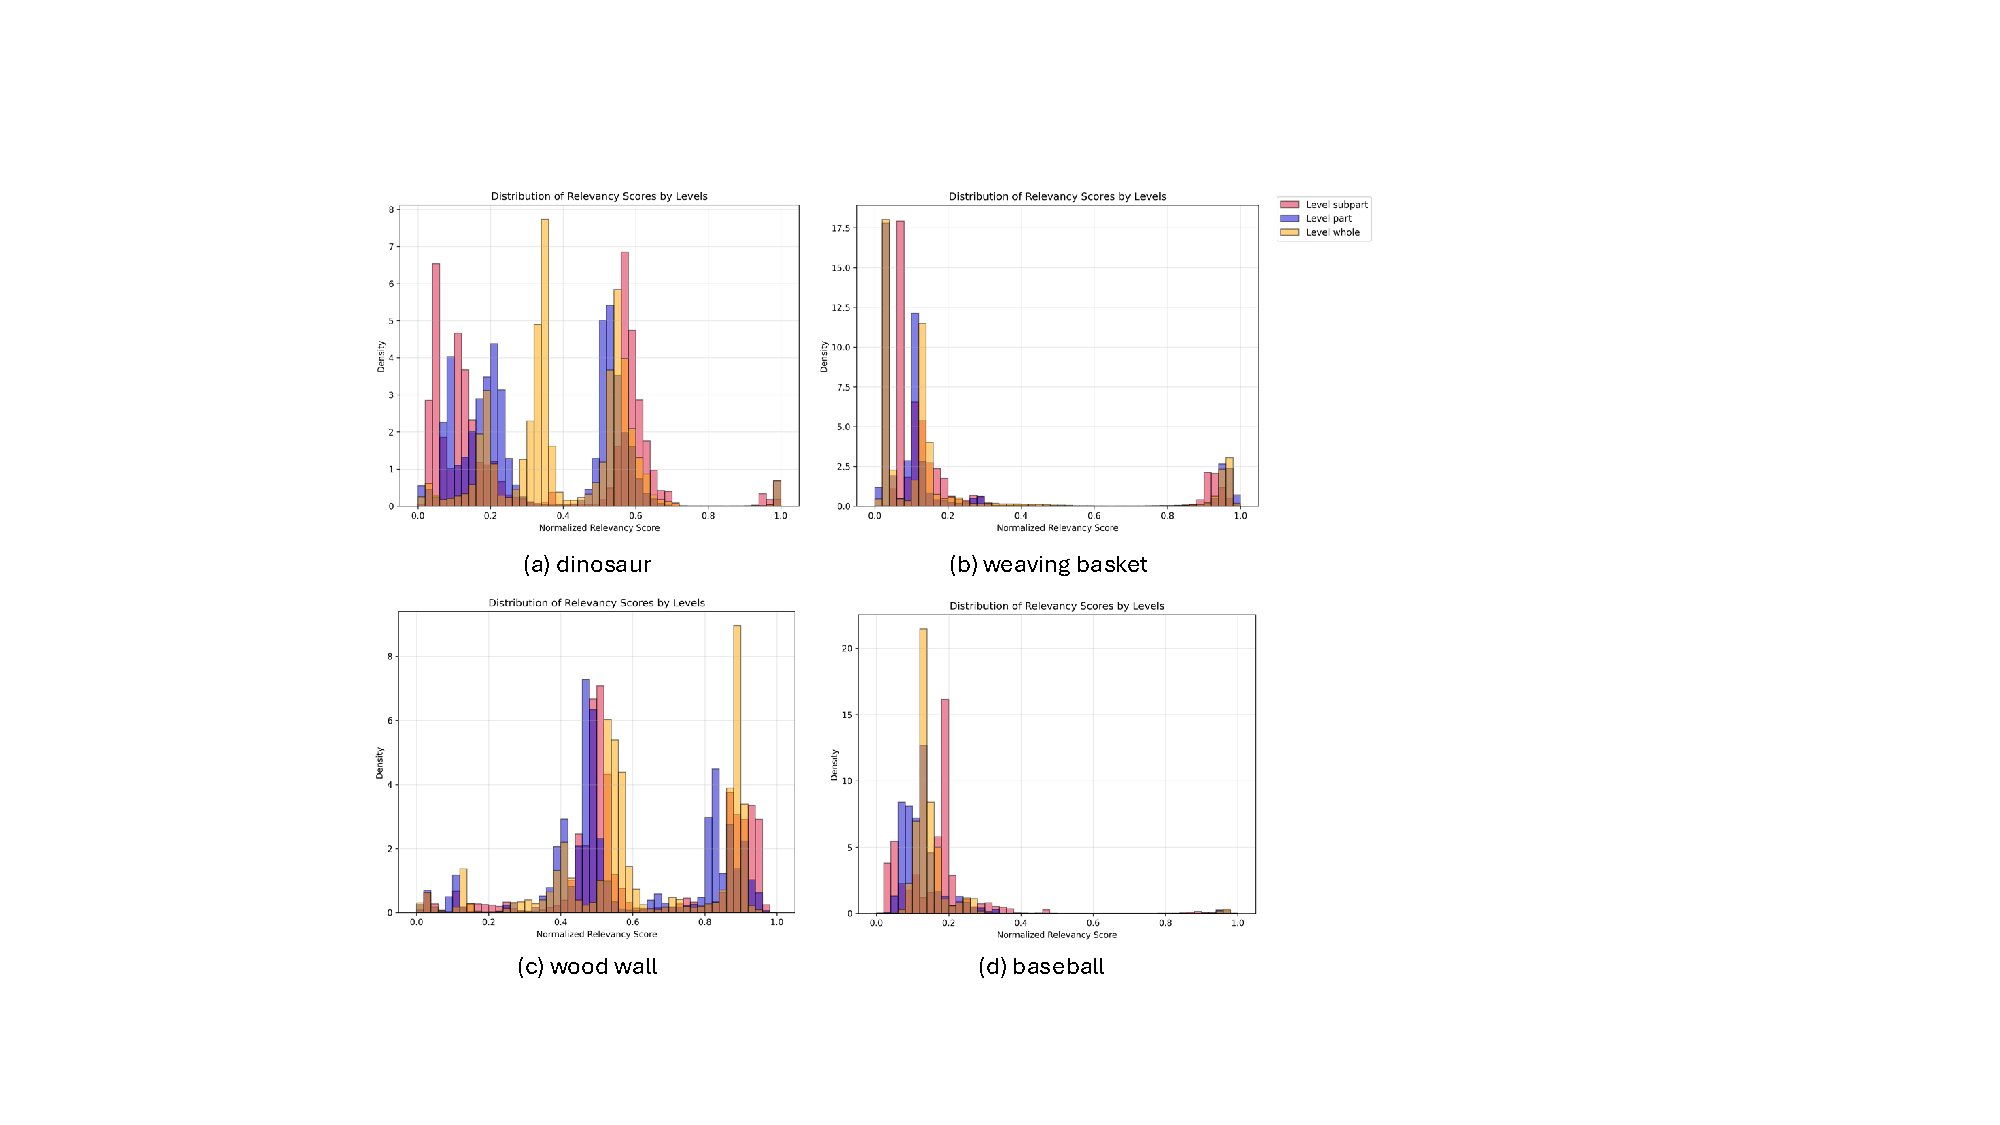
\includegraphics[trim={6cm 2.5cm 10cm 3cm}, clip, width=0.5\textwidth]{figures/distr_rele_score.pdf}
    \caption{Distribution of relevancy scores across hierarchical levels (subpart, part, and whole) when applying different queries to room scene in the 3D-OVS dataset. Each color represents a distinct hierarchical level, illustrating the distribution of relevancy scores at different hierarchies. }
    \label{fig:distr}
\end{figure}
We observe that different object queries yield varying ranges of relevancy scores, which makes it challenging to set a consistent threshold for object segmentation across query types, as shown in Figure~\ref{fig:distr}. To address this limitation, we propose a dynamic thresholding approach. 
For each query, we evaluate a range of threshold values with a step size of 0.01. At each threshold, we create a binary mask by selecting regions where the relevancy score exceeds the current threshold value, and compute the average relevancy score within this masked area. These average relevancy scores at different thresholds are plotted in Figure~\ref{fig:grad}, shown by the increasing trend lines.

Our goal is to identify a "stable region" where variations in the threshold minimally affect both the mask size and average relevancy score. Specifically, we find the region where the absolute gradient of the average relevancy score (the rate of change of average relevancy score with respect to different thresholds) is below the chosen stability threshold, as shown in Figure~\ref{fig:grad_w_thres}. We then select the middle value from this stable range as our final threshold for each different query, as illustrated in Figure~\ref{fig:grad}. The presence of a stable region indicates an object with consistent relevancy scores across threshold changes. In cases where multiple stable regions exist, we select the highest confidence prediction. We apply this improved evaluation methodology to the 3D-OVS dataset to ensure fair comparison across different query types.

\begin{figure}[!h]
    \centering
    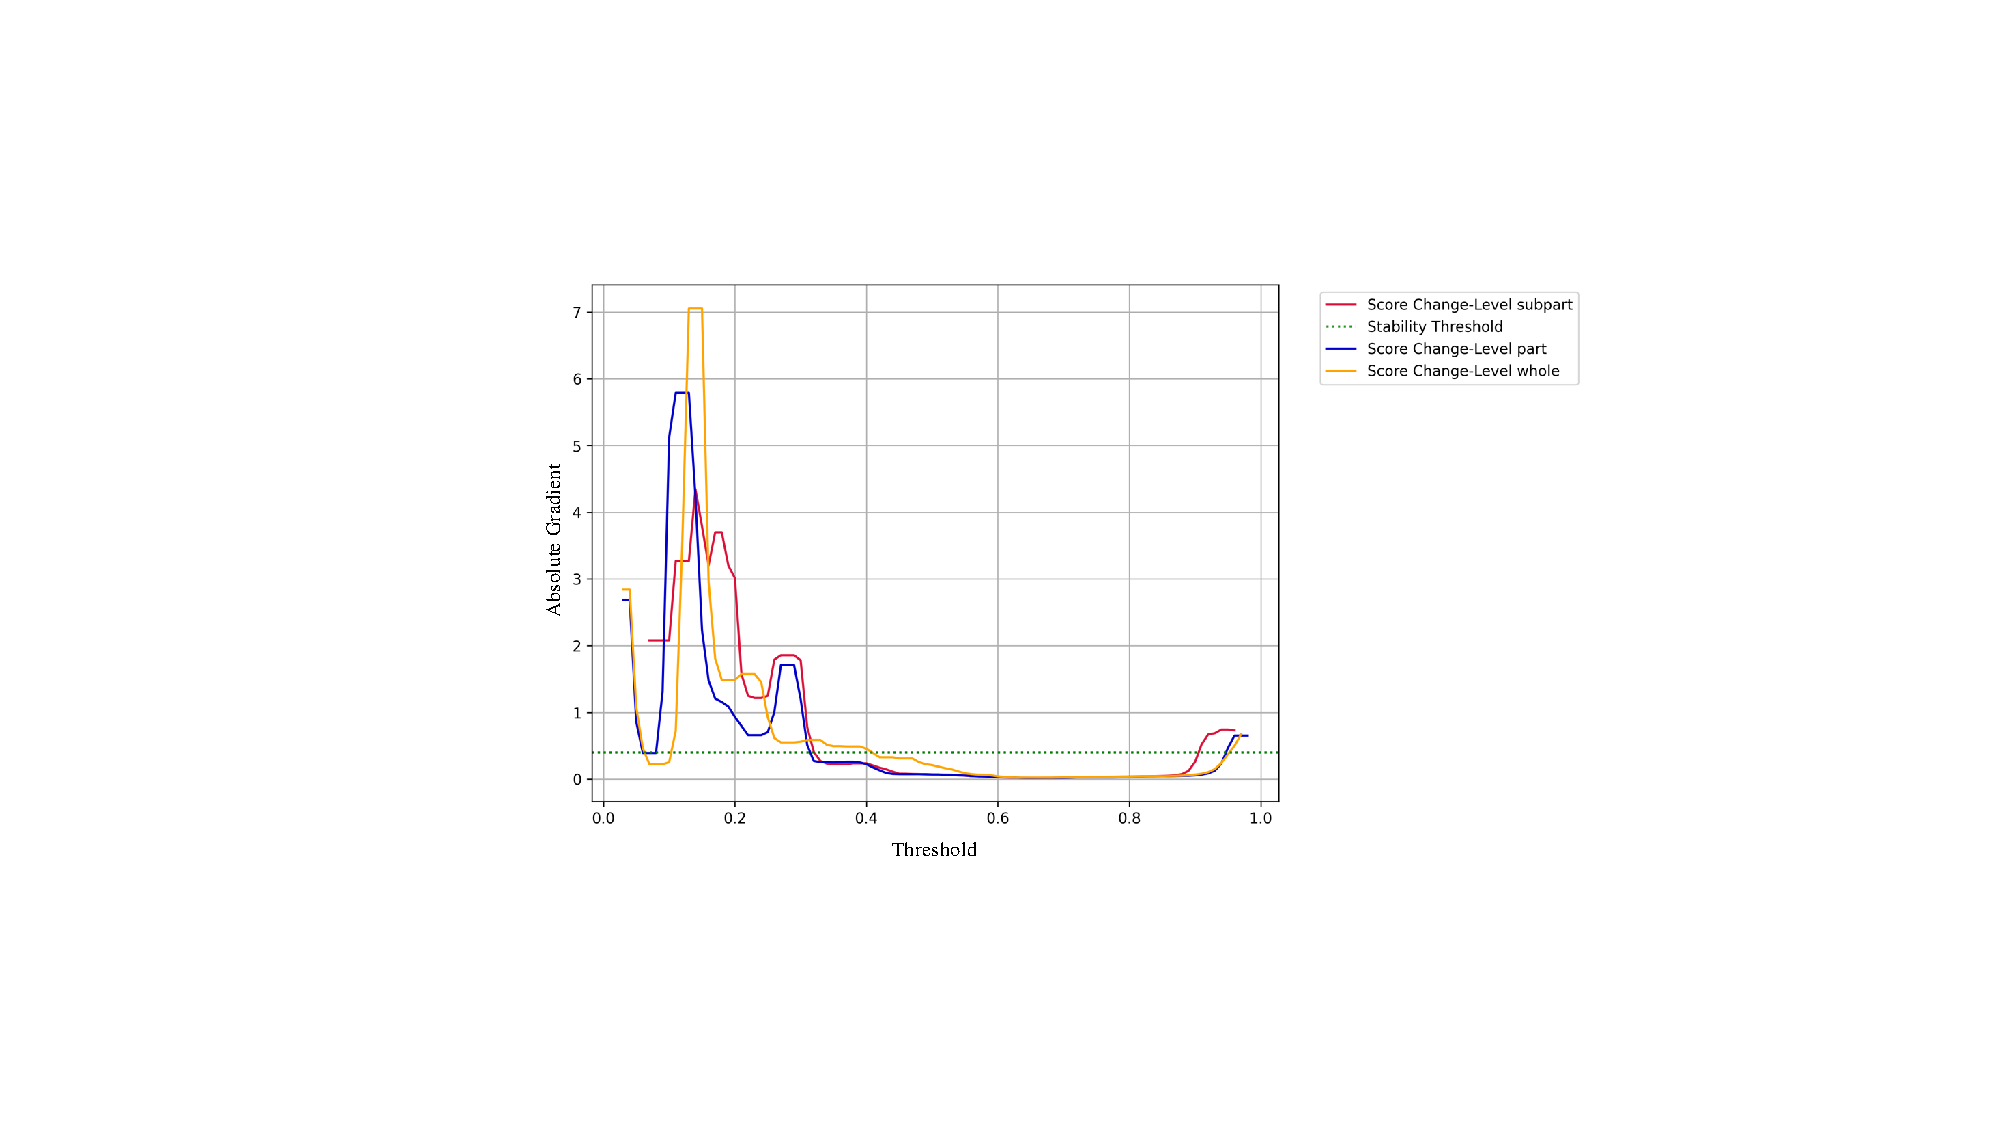
\includegraphics[trim={8cm 4cm 6cm 3cm}, clip, width=0.5\textwidth]{figures/grad_w_thres.pdf}
    \caption{Visualization of the absolute gradient of average relevancy scores. The gradient measures the rate of change in average relevancy scores across different thresholds. The green dotted line indicates the stability threshold, with lower gradient values corresponding to more stable regions. This plot corresponds to the "weaving basket" query in the room scene.}
    \label{fig:grad_w_thres}
\end{figure}

\begin{figure}[!h]
    \centering
    \vspace{-0.5cm}
    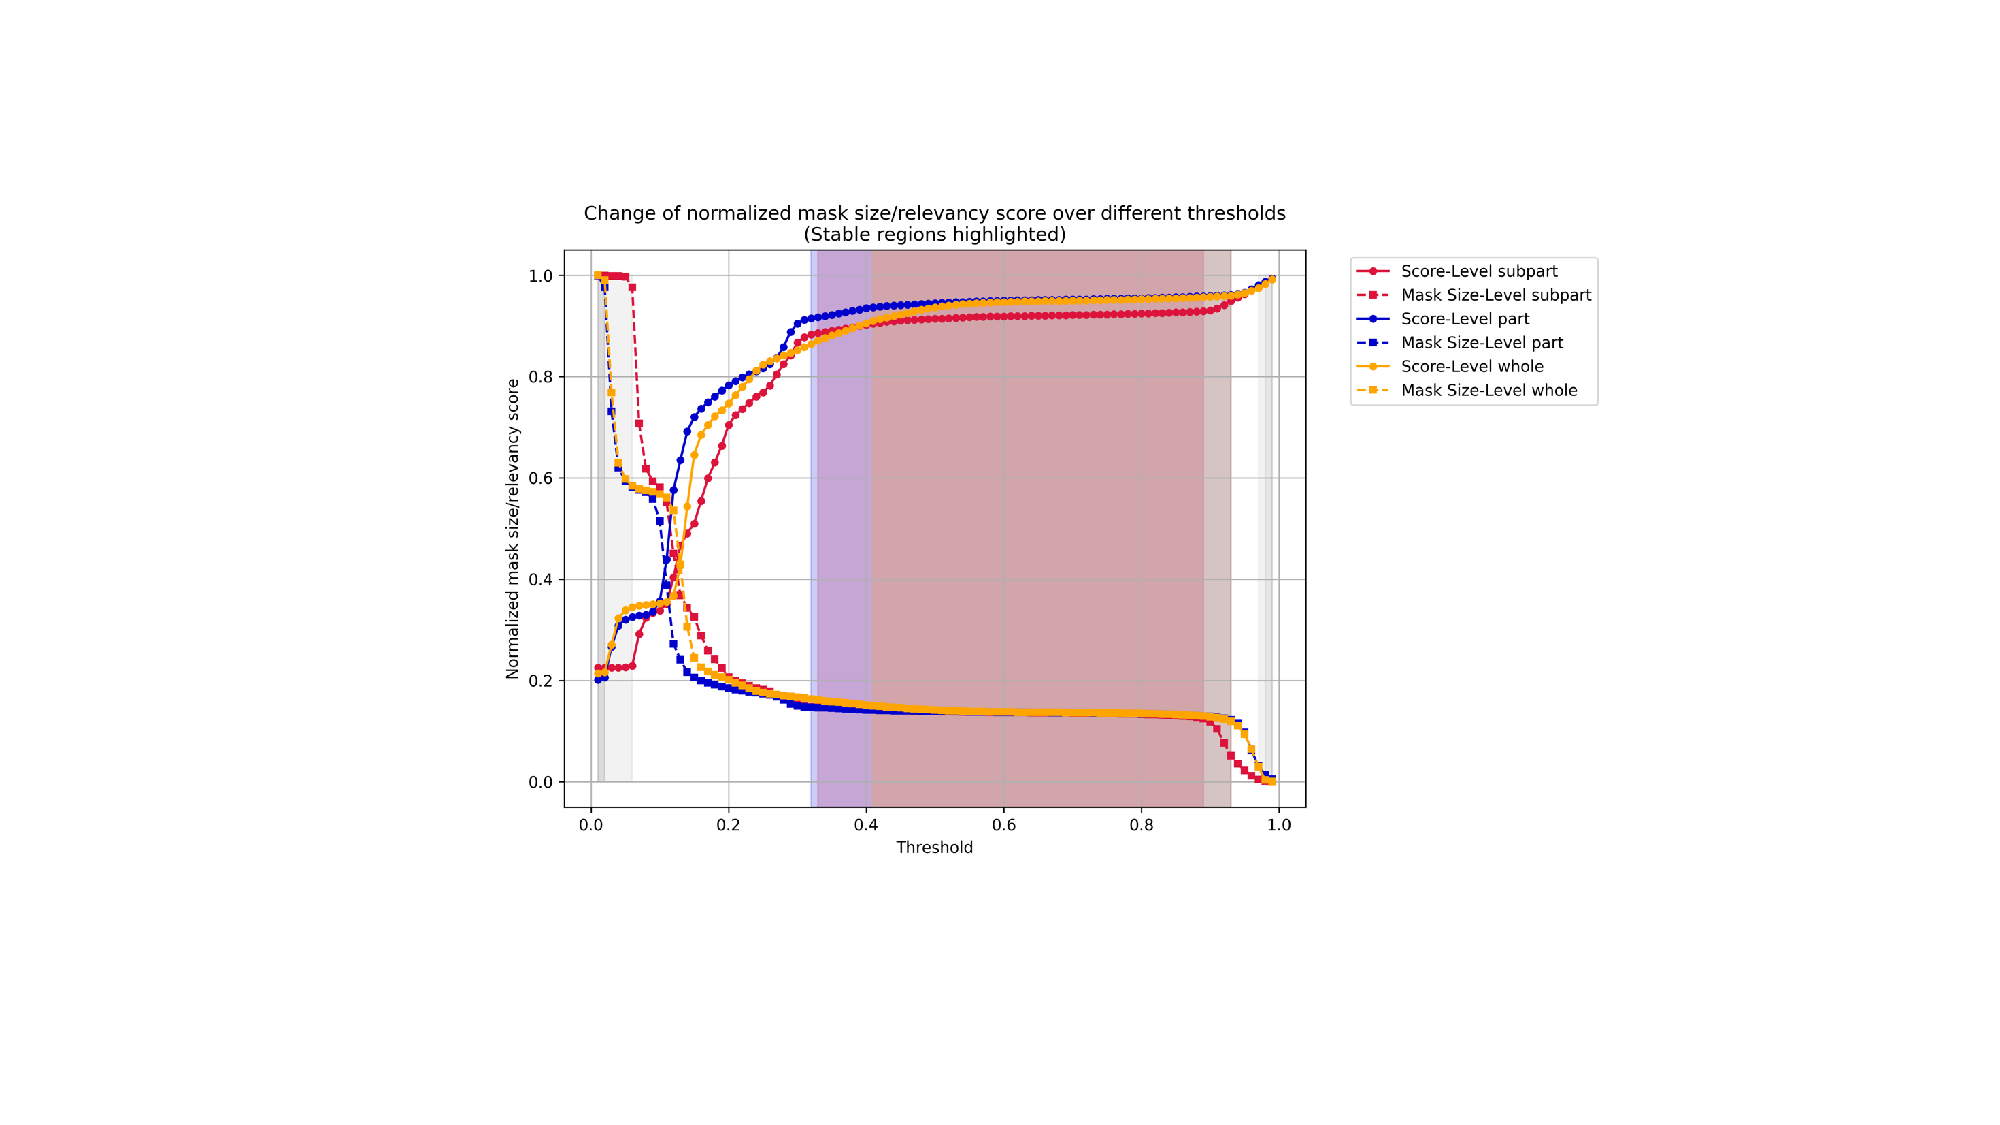
\includegraphics[trim={7cm 4cm 6cm 3cm}, clip, width=0.5\textwidth]{figures/grad.pdf}
    \caption{Relationship between score thresholds, normalized mask sizes, and relevancy scores for the "weaving basket" query in room scene. The plot shows how mask sizes decrease (downward trends with dotted lines) and average relevancy scores change (upward trends with smooth lines) as the threshold increases. Different hierarchical levels are represented by distinct colors, with the shaded region indicating the optimal stable region identified by our stability threshold.}
    \label{fig:grad}
\end{figure}

\section{Additional Visualizations}
\subsection{LERF Visualization}
We show additional visualization of the semantic features on LERF Dataset in Figure~\ref{fig:lerf-vis3}.

\begin{figure}[t]
    \centering
    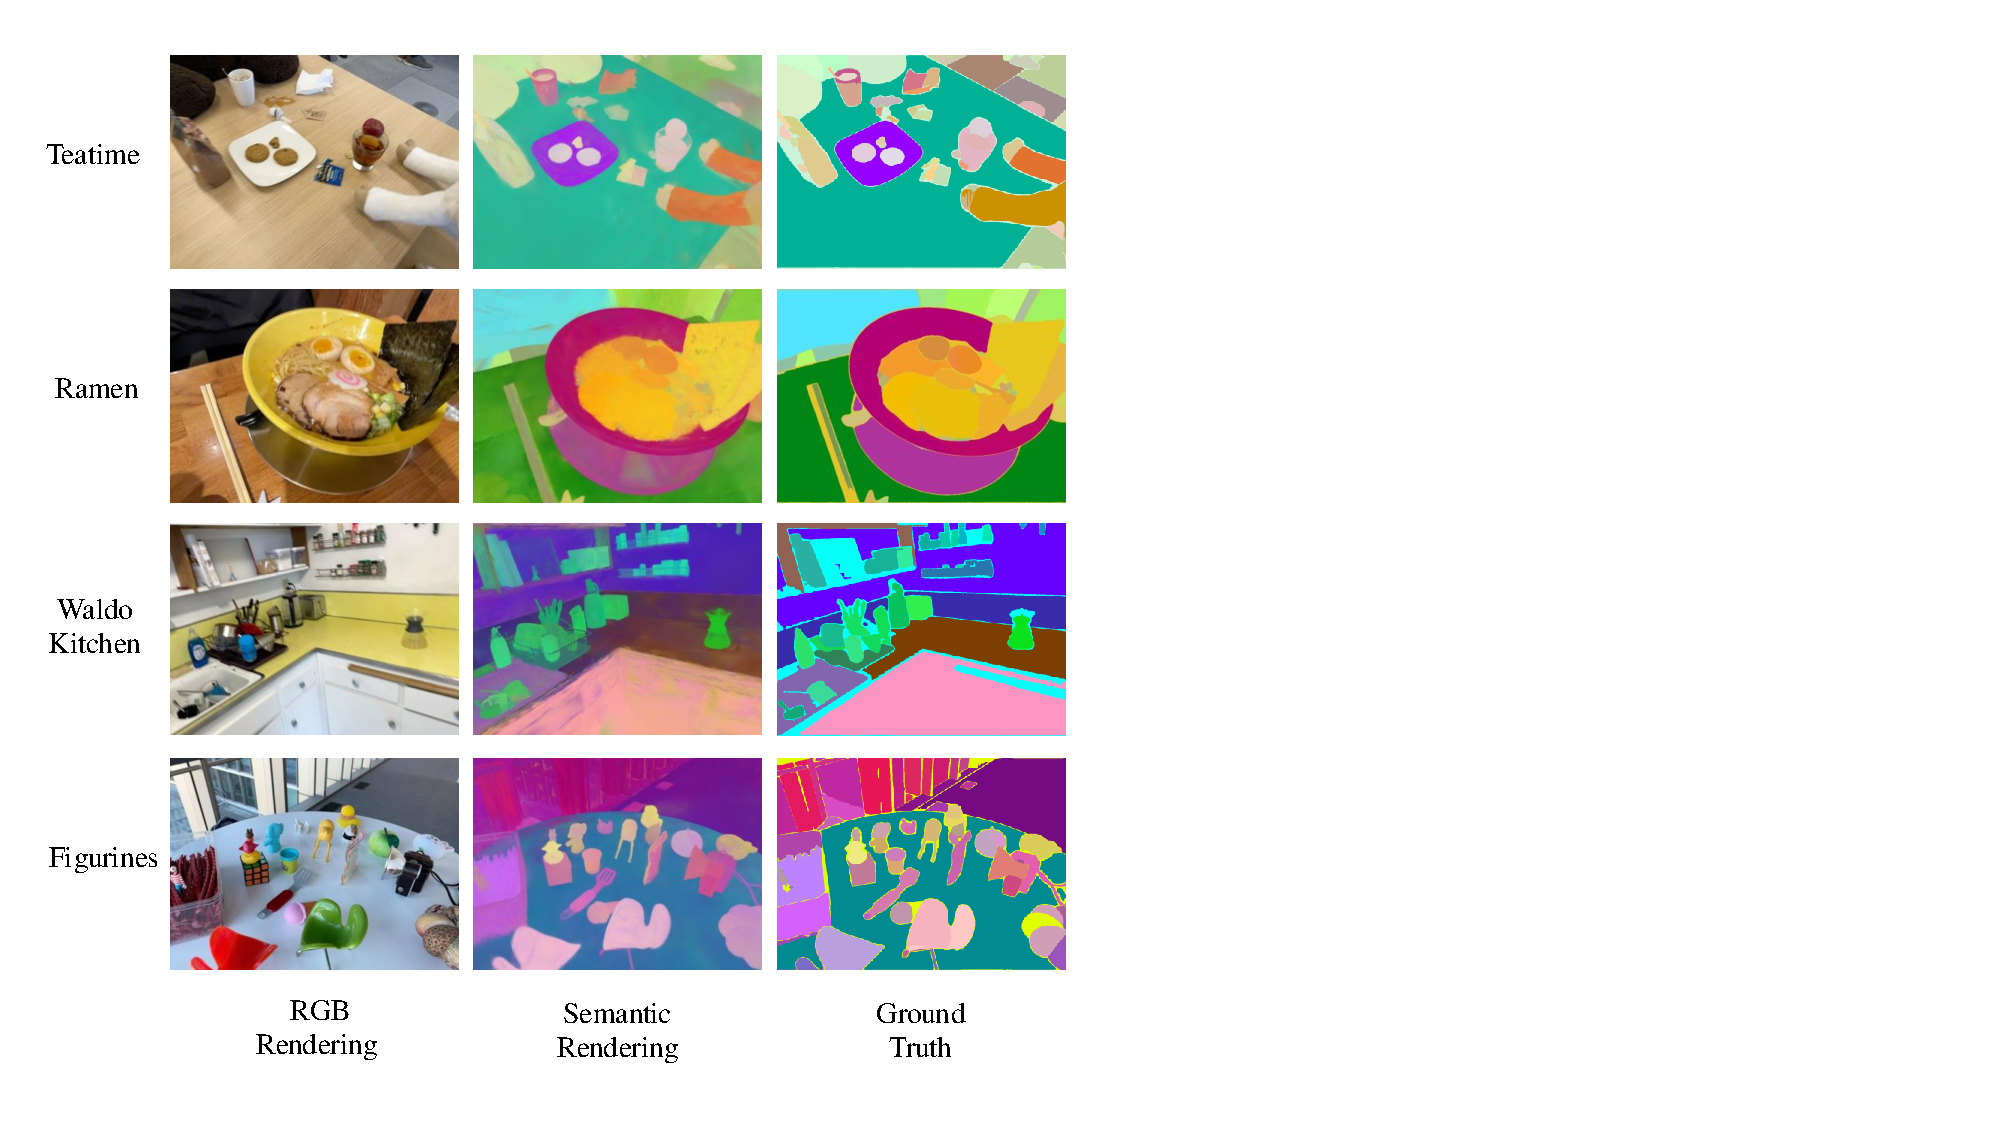
\includegraphics[width=0.88\textwidth]{figures/lerf_vis3.pdf}
    \caption{PCA visualization of semantic features on LERF Dataset. (a) Original RGB rendering. (b) PCA visualization of our rendered semantic feature maps. (c) Initial semantic feature maps extracted using CLIP from SAM segmentations. }
    \label{fig:lerf-vis3}
\end{figure}

\subsection{3DOVS Visualization}
We show more examples on the 3D-OVS dataset in Figure~\ref{fig:room},~\ref{fig:bench}, and ~\ref{fig:lawn}.
\begin{figure*}[t]
    \centering
    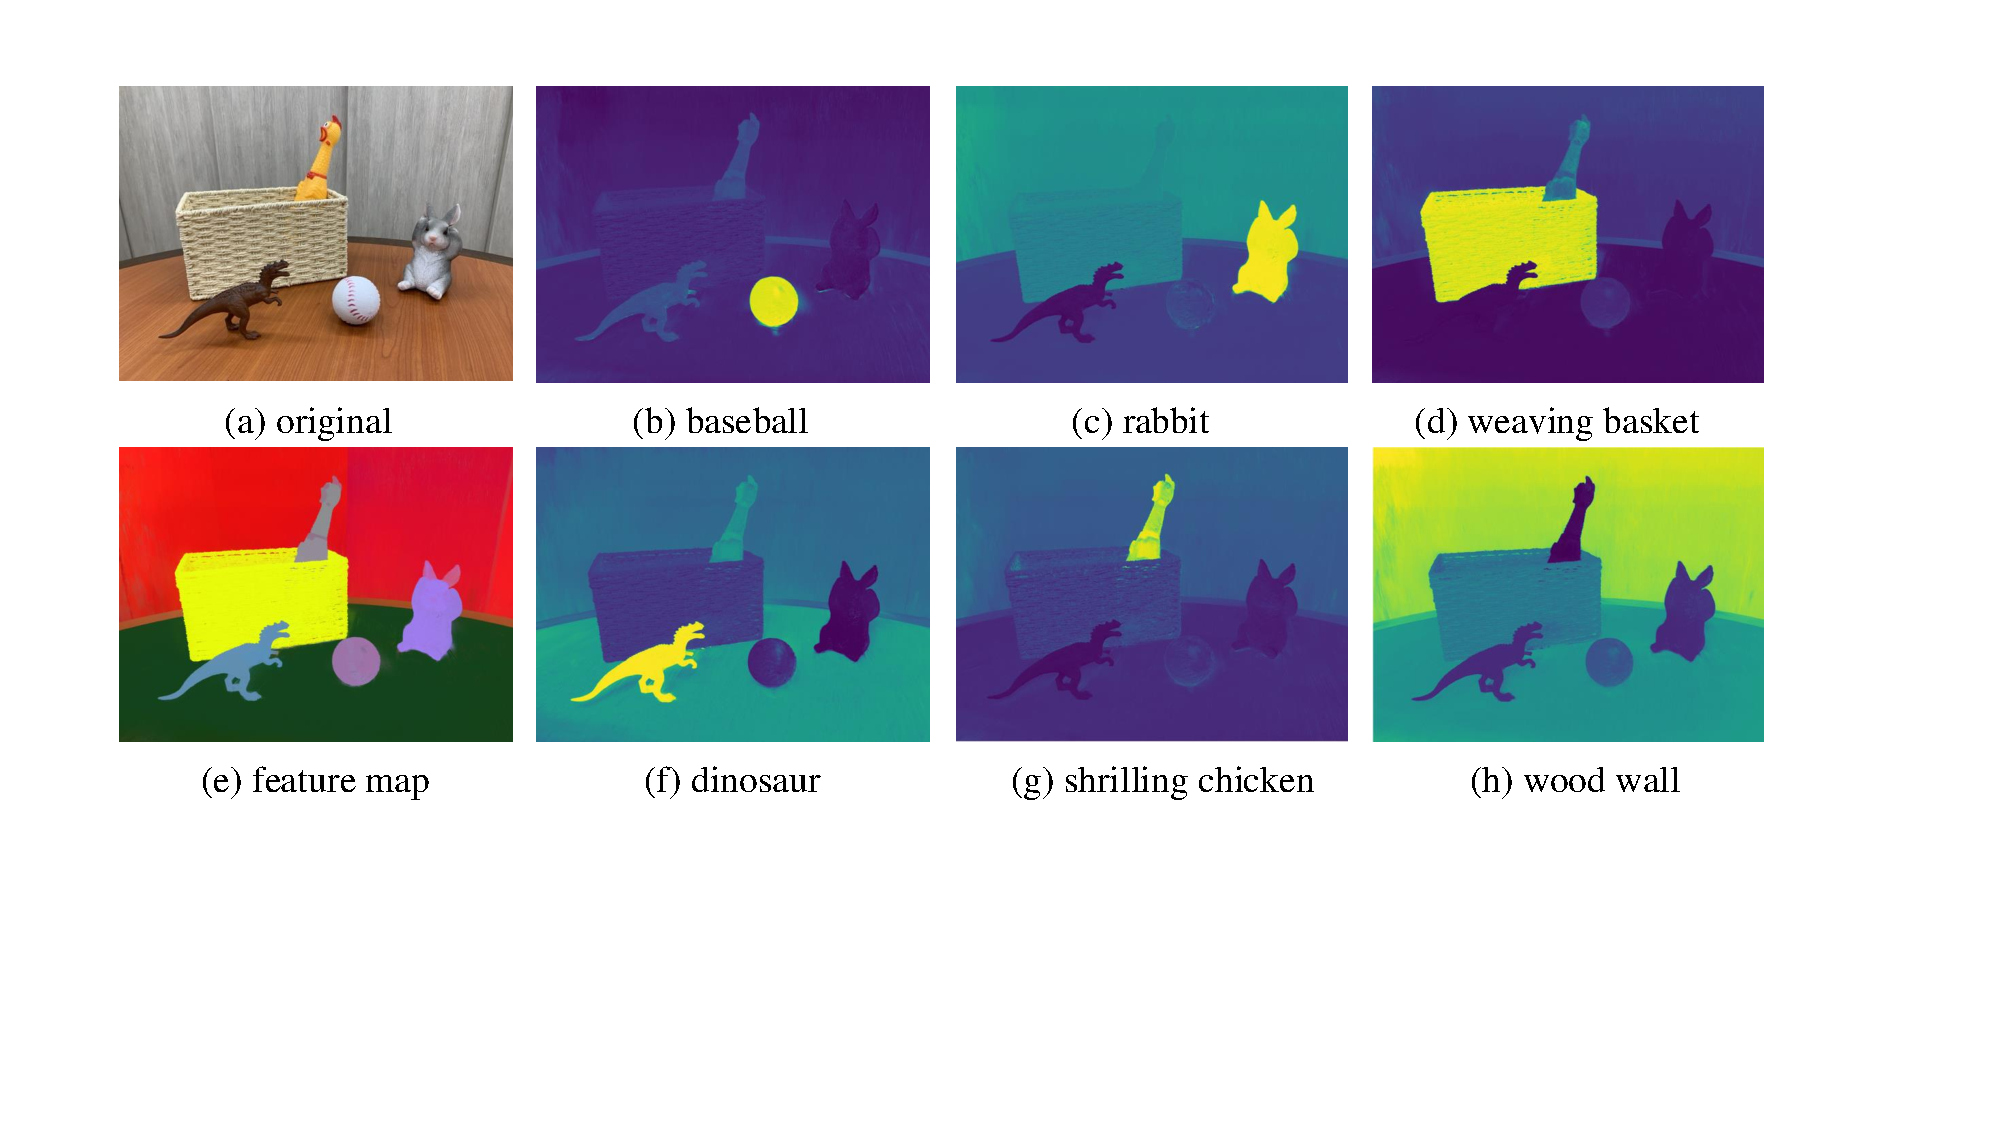
\includegraphics[trim={1cm 5cm 3cm 0.5cm}, clip, width=0.8\textwidth]{figures/room.pdf}
    \caption{3D-OVS: room}
    \label{fig:room}
\end{figure*}
\begin{figure*}[t]
    \centering
    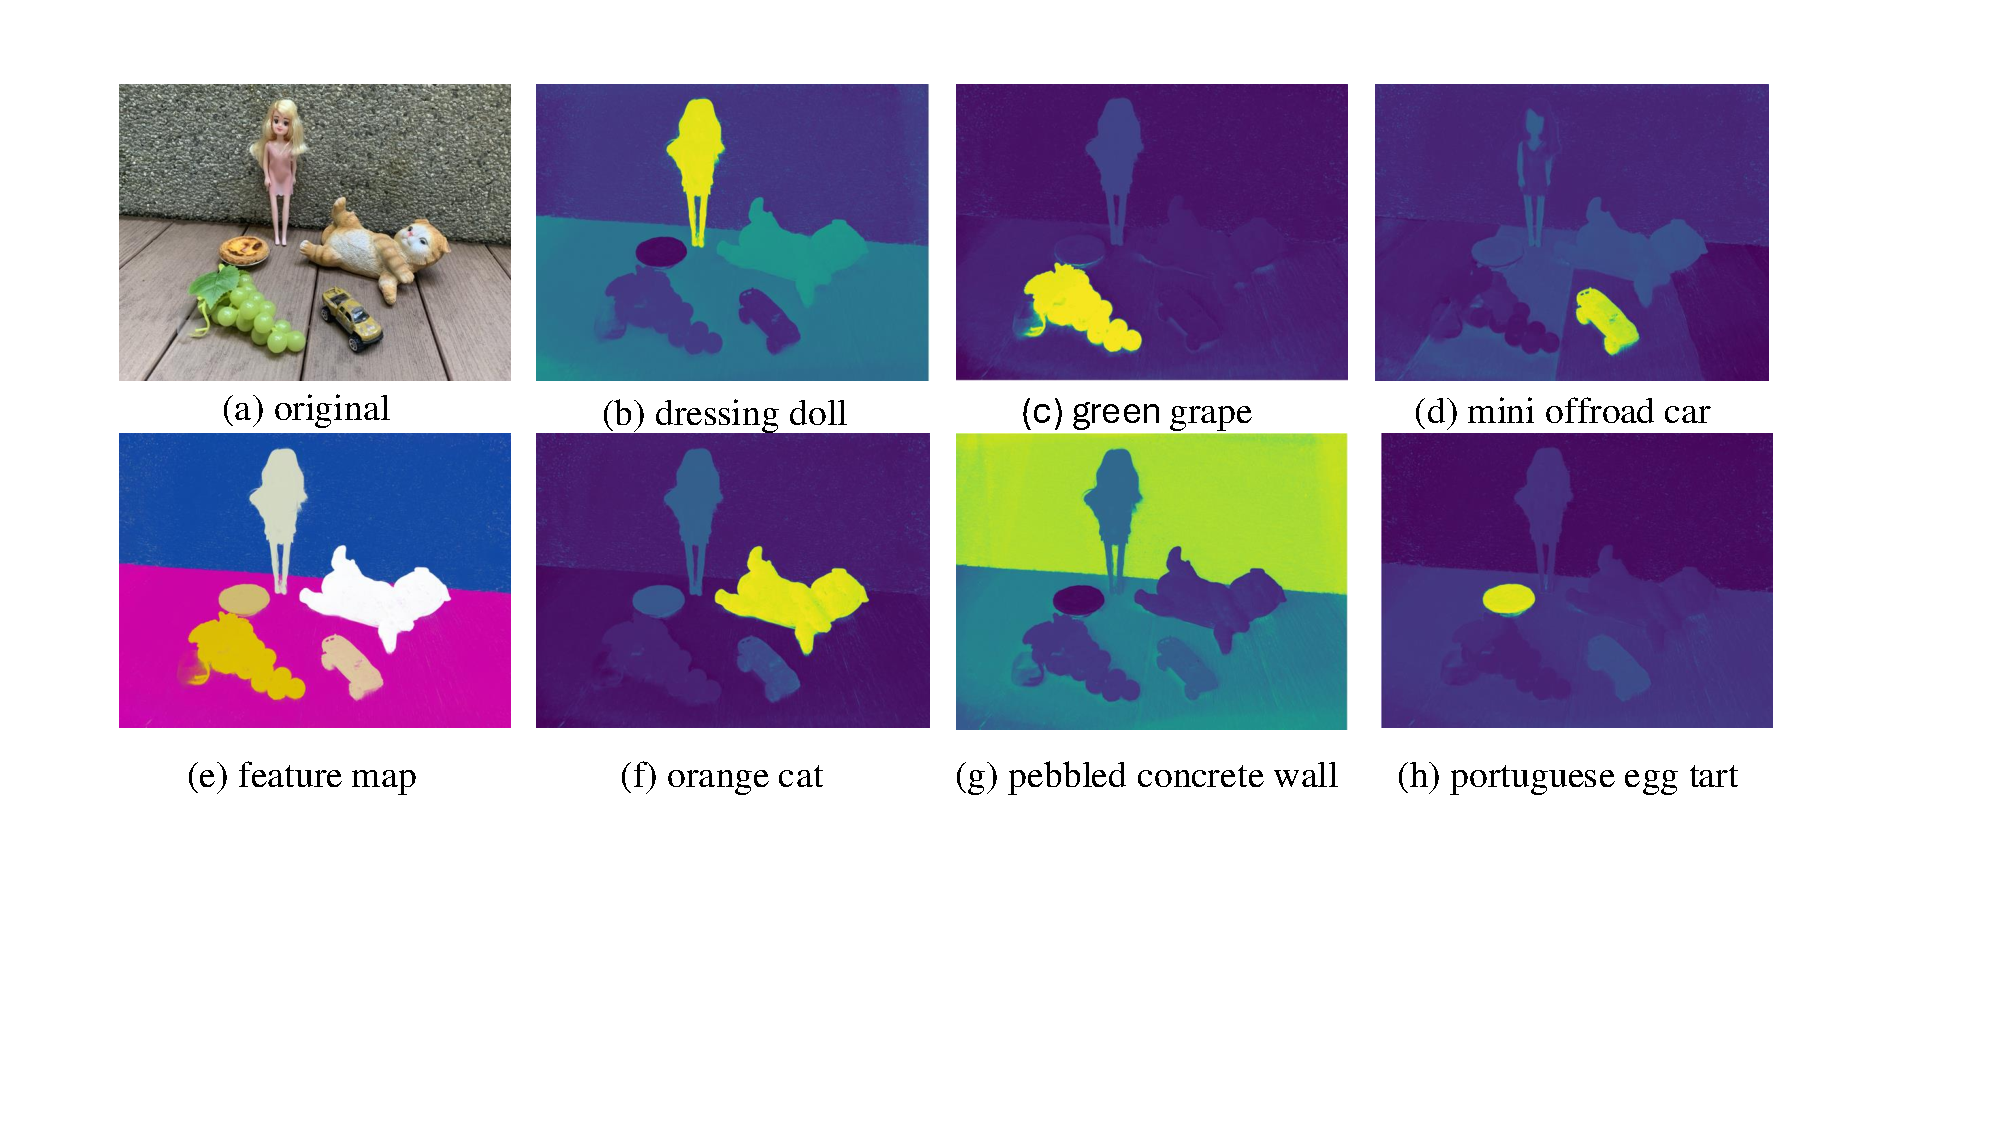
\includegraphics[trim={1cm 5cm 3cm 0.5cm}, clip, width=0.8\textwidth]{figures/bench.pdf}
    \caption{3D-OVS: bench}
    \label{fig:bench}
\end{figure*}
\begin{figure*}[t]
    \centering
    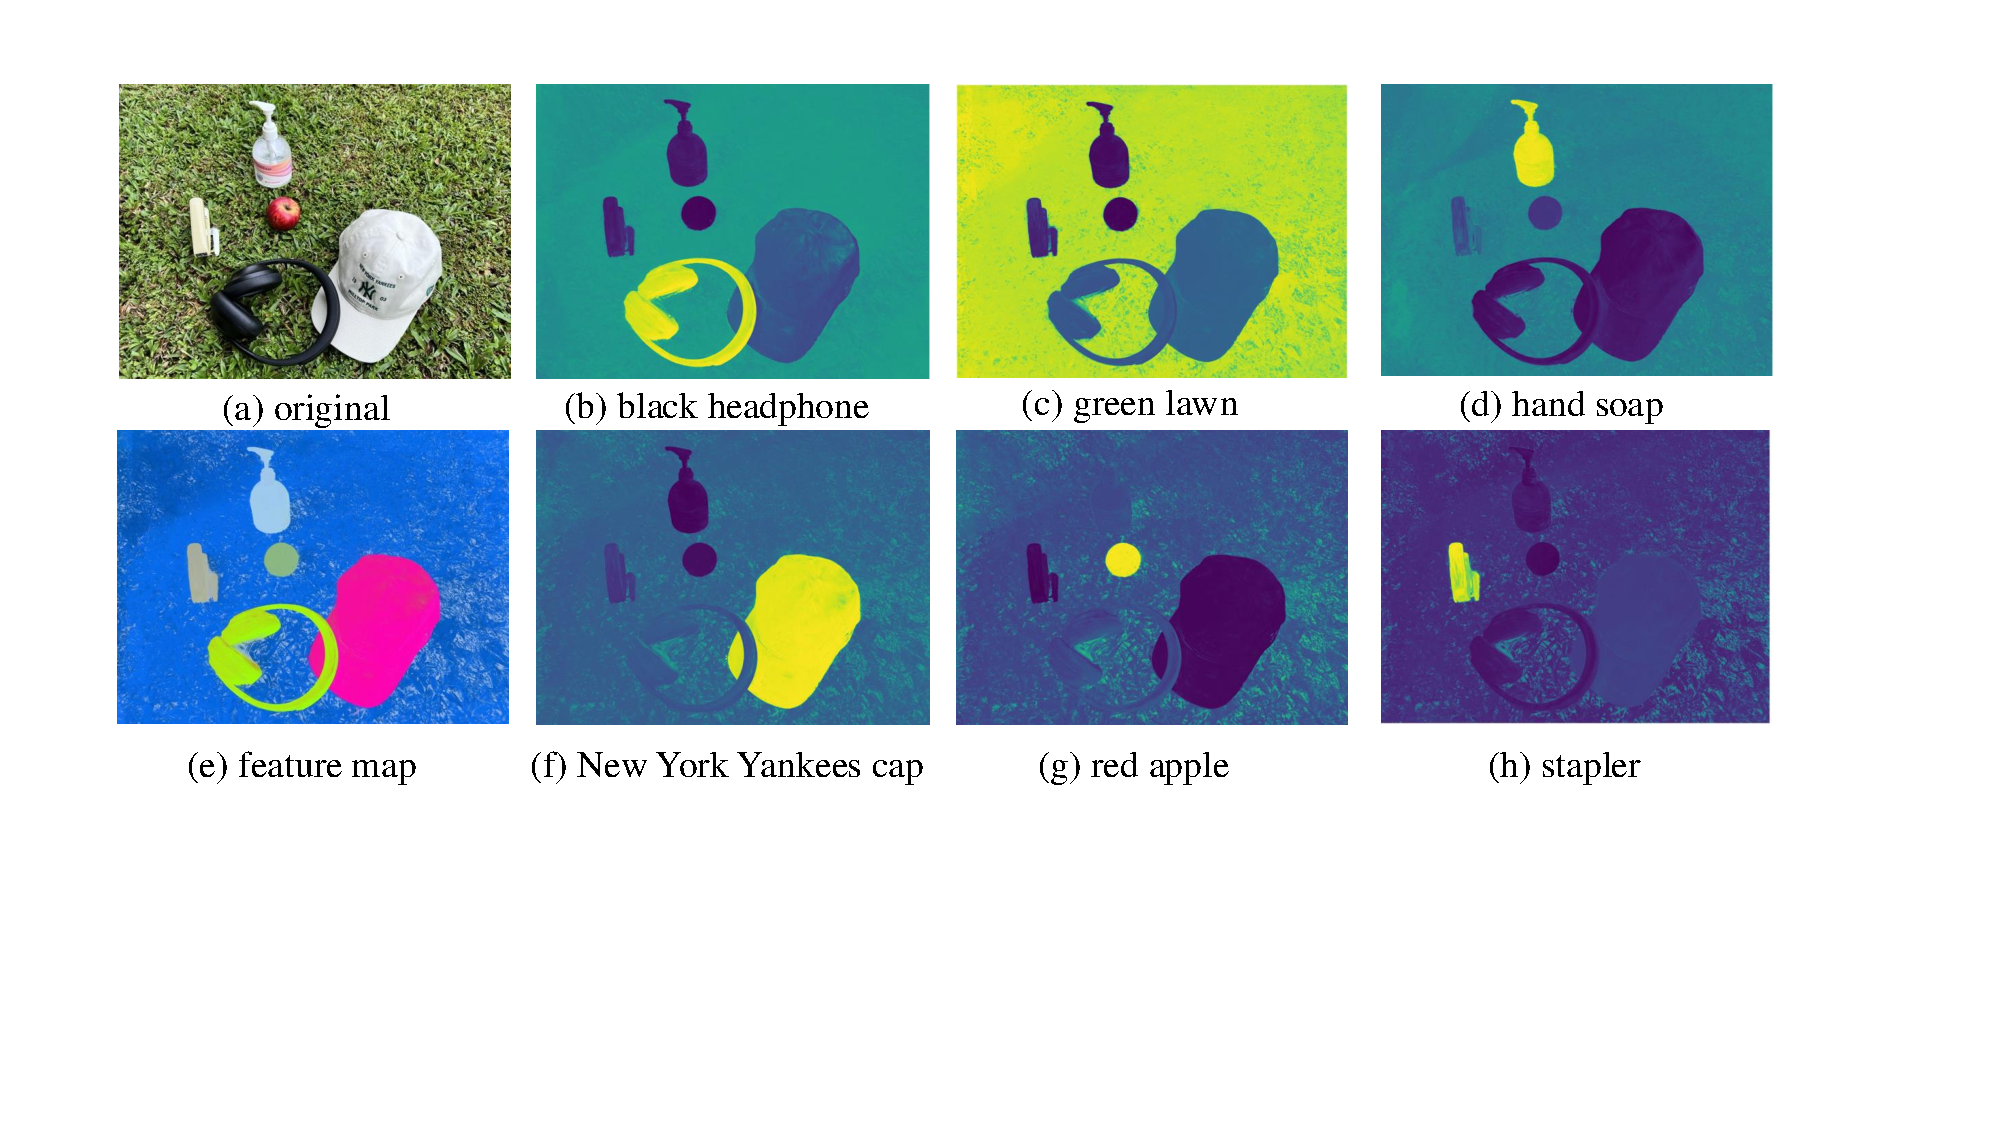
\includegraphics[trim={1cm 5cm 3cm 0.5cm}, clip, width=0.8\textwidth]{figures/lawn.pdf}
    \caption{3D-OVS: lawn}
    \label{fig:lawn}
\end{figure*}







% \section{Version2 Joanna}

% For LGS with uniformly distributed language features $p(f)$, which we assume for the efficient feature space of CLIP, the estimator is equivalent to the Maximum Likelihood (ML) $\arg\max_f p(x|f)$. This simplification is possible because with a uniform prior, the $p(f)$ term becomes constant and doesn't affect the optimization, while $p(x)$ is also constant with respect to $f$.

% This function can be evaluated separately for each pixel $x_{p,v}$ at view $v$ under conditional independence given the surface $f$: 
% \begin{equation}
%      \arg\max_f p(x|f) =  \arg\max_f \prod_{v=1}^V \prod_{p \in P_v} p(x_{p,v}|f)
% \end{equation}
% where $P_v$ is the set of pixels in view $v$ on which Gaussian influences.

% We formulate the ML of LGS with the following noise model: 
% Noise of language features due to varying object appearance as IID normal distributed $\epsilon_{p,v} \sim \mathcal{N}(\mathbf{0}, \sigma^2\mathbf{I})$. This represents the inherent uncertainty in the 2D features extracted from different viewpoints.

% Hence, the rendered 2D feature at pixel $p$ in view $v$ is:
% \begin{equation}
%     x_{p,v} = \sum_{i=1}^R w_{i,p,v}f_i + \epsilon_{p,v}
% \end{equation}
% where $R$ is the number of Gaussians along the ray, $\epsilon_{p,v}$ is the language feature noise, and $w_{i,p,v}$ is the alpha blending weight for Gaussian $i$ at pixel $p$ in view $v$ defined below:
% \begin{equation}
%     w_{i,p,v} = \alpha_i \prod_{j=1}^{i-1}(1-\alpha_j)
% \end{equation}

% To solve $\arg\max_f p(x|f)$, we first take the logarithm of the likelihood function, which transforms the product into a sum and simplifies the optimization:
% \begin{align}
%     \log p(x|f) &= \log \prod_{v=1}^V \prod_{p \in P_v} p(x_{p,v}|f) \\
%     &= -\frac{1}{2\sigma^2} \sum_{v,p} \left\| x_{p,v} - \sum_{i=1}^R w_{i,p,v}f_i \right\|^2 + \text{const.}
% \end{align}

% Taking derivative with respect to $f_i$, 3D language feature of Gaussian $i$:
% \begin{align}
%     \frac{\partial \log p}{\partial f_i} &= \frac{1}{\sigma^2} \sum_{v,p} w_{i,p,v} \left( x_{p,v} - \sum_{k=1}^R w_{k,p,v}f_k \right) = 0 \\
%     \Rightarrow \sum_{v,p} w_{i,p,v}x_{p,v} &= \sum_{k=1}^R \left( \sum_{v,p} w_{i,p,v}w_{k,p,v} \right)f_k
% \end{align}
% The left side is the weighted sum of observed 2D features, while the right side captures how Gaussians interact in the rendering process.

% \subsection{Practical Simplification}
% Here, given the properties of 3D Gaussian Splatting, we make the following assumptions to simplify the formula:
% \begin{enumerate}
%     \item[(a)] Sparse Influence: Assuming that for most pixels, only one Gaussian has significant influence (weight close to 1) means that the rendering is dominated by non-overlapping Gaussians.
%     \item[(b)] Negligible Cross-Talk: This explicitly states that the product of weights from different Gaussians at the same pixel is approximately zero, which directly gives us:
%     $w_{i,p,v}w_{k,p,v} \approx 0$ for $i \neq k$. This eliminates the cross-terms in our equation.
%     \item[(c)] Binary Approximation: If weights are approximately binary (either close to 0 or close to 1), then $w_{k,p,v}^2 \approx w_{k,p,v}$. This would give $w_{i,p,v}^2 \approx w_{i,p,v}$.
% \end{enumerate}

% With these assumptions, the system of equations simplifies dramatically. When $i \neq k$, the corresponding terms become negligible, and when $i = k$, we get:
% \begin{align}
% \sum_{v,p} w_{i,p,v}x_{p,v} &\approx \left( \sum_{v,p} w_{i,p,v}^2 \right)f_i \\
% &\approx \left( \sum_{v,p} w_{i,p,v} \right)f_i \quad \text{(using assumption (c))}
% \end{align}

% Therefore, equation can be simplified to the closed-form solution below:
% \begin{equation}
%     \boxed{
%         f_i = \frac{\sum\limits_{v=1}^V \sum\limits_{p \in P_v} w_{i,p,v}x_{p,v}}{\sum\limits_{v=1}^V \sum\limits_{p \in P_v} w_{i,p,v}}
%     }
% \end{equation}
% This formula has an intuitive interpretation: the optimal 3D feature for each Gaussian is a weighted average of the 2D features observed at pixels where the Gaussian has influence, with weights proportional to the Gaussian's contribution to each pixel.

% For practical implementation, we introduce one additional key assumption: The Gaussian's maximum influence occurs at its projected mean in most cases. This allows us to focus computation only on the most relevant pixels: 
% \begin{equation}
%     \boxed{
%         f_i = \frac{\sum\limits_{s \in S} w_{i}^s x^s}{\sum\limits_{s \in S} w_{i}^s}
%     }
% \end{equation}
% where $S$ denotes the set of pixels across all views where Gaussian $i$ is visible, $w_i^s$ represents the alpha blending weight of Gaussian $i$ at its single projected pixel location in view $s$, and $x^s$ is the 2D feature vector observed at the pixel where Gaussian $i$
% projects in view $s$.

% This further simplification focuses only on the direct projection of each Gaussian in each view, rather than all pixels where it might have some influence. It substantially reduces computation while maintaining the theoretical foundation of our approach.



% \section{Original Proof}
% \subsection{Notations}
% \begin{itemize}
%     \item $x \in \mathbb{R}^d$: 2D CLIP feature vector (observed)
%     \item $f_i \in \mathbb{R}^d$: 3D CLIP feature vector of $i$-th Gaussian
%     \item $x_{p,v}$: Feature at pixel $p$ in view $v$
%     \item $w_{i,p,v}$: Alpha blending weight for Gaussian $i$ at pixel $p$ in view $v$
%     \item $\alpha_i$: Opacity of $i$-th Gaussian
%     \item $\epsilon_{p,v} \sim \mathcal{N}(0, \sigma^2\mathbf{I})$: Observation noise
%     \item $V$: Number of camera views
%     \item $P_v$: Set of pixels in view $v$
%     \item $R$: Number of 3D Gaussians
%     \item $\prod_{j=1}^{i-1}(1-\alpha_j)$: Occlusion accumulation term
% \end{itemize}

% We establish our framework with four key assumptions:
% \begin{enumerate}[label=(\roman*)]
%     \item \textbf{Uniform Prior}: The language features in CLIP space have uniform distribution:
%     \[
%     p(f) \propto \text{constant}
%     \]
%     making MAP estimation equivalent to ML:
%     \[
%     \arg\max_{f} p(f|x) = \arg\max_{f} p(x|f)
%     \]
    
%     \item \textbf{Conditional Independence}: Pixel observations are conditionally independent given 3D features $f$:
%     \[
%     p(x|f) = \prod_{v=1}^V \prod_{p \in P_v} p(x_{p,v}|f)
%     \]
    
%     \item \textbf{Noise Characteristics}:
%     \begin{itemize}
%         \item Feature noise: $\epsilon_{p,v} \sim \mathcal{N}(\mathbf{0}, \sigma^2\mathbf{I})$
%         \item Projection approximated by Gaussian mixtures
%     \end{itemize}
    
%     \item \textbf{Alpha Blending Weights}:
%     \[
%     w_{i,p,v} = \alpha_i \prod_{j=1}^{i-1}(1-\alpha_j)
%     \]
%     encoding occlusion relationships between Gaussians.
% \end{enumerate}

% \subsection{Forward Observation Model}
% The rendered 2D feature at pixel $p$ in view $v$ is:
% \begin{equation}
%     x_{p,v} = \sum_{i=1}^R w_{i,p,v}f_i + \epsilon_{p,v}
% \end{equation}
% where $R$ is the number of Gaussians along the ray and $\epsilon_{p,v}$ the Observation noise.

% \subsection{Likelihood Formulation}
% \subsubsection{Per-Pixel Likelihood}
% For a single observation:
% \begin{equation}
%     p(x_{p,v}|f) = \frac{1}{(2\pi\sigma^2)^{d/2}} \exp\left(-\frac{1}{2\sigma^2} \left\| x_{p,v} - \sum_{i=1}^R w_{i,p,v}f_i \right\|^2 \right)
% \end{equation}

% \subsubsection{Complete Log-Likelihood}
% Aggregating over all views and pixels:
% \begin{equation}
%     \log p(x|f) = -\frac{1}{2\sigma^2} \sum_{v,p} \left\| x_{p,v} - \sum_{i=1}^R w_{i,p,v}f_i \right\|^2 + \text{const.}
% \end{equation}

% \subsection{Maximum Likelihood Estimation}
% \subsubsection{First-Order Condition}
% Taking derivative with respect to $f_k$:
% \begin{align}
%     \frac{\partial \log p}{\partial f_k} &= \frac{1}{\sigma^2} \sum_{v,p} w_{k,p,v} \left( x_{p,v} - \sum_{i=1}^R w_{i,p,v}f_i \right) = 0 \\
%     \Rightarrow \sum_{v,p} w_{k,p,v}x_{p,v} &= \sum_{i=1}^R \left( \sum_{v,p} w_{k,p,v}w_{i,p,v} \right)f_i
% \end{align}

% \subsection{Simplification via 3DGS Properties}
% \begin{enumerate}[label=(\alph*)]
%     \item \textbf{Sparse Influence}: $\exists! i$ s.t. $w_{i,p,v} \approx 1$ for most pixels
%     \item \textbf{Negligible Cross-Talk}: $w_{i,p,v}w_{j,p,v} \approx 0$ for $i \neq j$
%     \item \textbf{Binary Approximation}: $w_{i,p,v}^2 \approx w_{i,p,v}$
% \end{enumerate}

% Under these conditions:
% \begin{equation}
%     \sum_{v,p} w_{k,p,v}x_{p,v} \approx \left( \sum_{v,p} w_{k,p,v} \right)f_k
% \end{equation}

% \subsection{Closed-Form Solution}
% Solving for $f_k$ gives:
% \begin{equation}
%     \boxed{
%         f_k = \frac{\sum\limits_{v=1}^V \sum\limits_{p \in P_v} w_{k,p,v}x_{p,v}}{\sum\limits_{v=1}^V \sum\limits_{p \in P_v} w_{k,p,v}}
%     }
% \end{equation}

% \subsubsection{Computational Efficiency Constraint}
% For practical implementation, we introduce one key assumption:

% \begin{enumerate}
%     \item \textbf{Center Dominance}: The Gaussian's maximum influence occurs at its projected mean:
%     \[
%     w_{k,p,v} \leq w_{k,\mathcal{C}_{k,v}} \quad \forall p \neq \mathcal{C}_{k,v}
%     \]
%     where $\mathcal{C}_{k,v}$ is the center pixel for Gaussian $k$ in view $v$.
% \end{enumerate}

% \subsubsection{Single-Pixel Approximation}
% Under these assumptions, we approximate:
% \begin{align*}
%     \sum_{p \in P_v} w_{k,p,v}x_{p,v} &\approx w_{k,\mathcal{C}_{k,v}}x_{\mathcal{C}_{k,v}} \\
%     \sum_{p \in P_v} w_{k,p,v} &\approx w_{k,\mathcal{C}_{k,v}}
% \end{align*}

% \subsubsection{Final Simplified Form}
% The closed-form solution reduces to:
% \begin{equation}
%     \boxed{
%         f_k^{\text{center}} = \frac{\sum\limits_{v=1}^V w_{k,\mathcal{C}_{k,v}}x_{\mathcal{C}_{k,v}}}{\sum\limits_{v=1}^V w_{k,\mathcal{C}_{k,v}}}
%     }
% \end{equation}

% \subsection{Interpretation}
% The estimator:
% \begin{itemize}
%     \item Computes visibility-weighted average of 2D features
%     \item Naturally handles occlusion through alpha blending weights
%     \item Maintains multi-view consistency via view aggregation
%     \item Preserves CLIP semantics through linear combination
% \end{itemize}

% This derivation provides a mathematically rigorous foundation for uplifting 2D language features to 3D Gaussians while respecting the rendering mechanics of 3D Gaussian Splatting.


